% =====================================================================
% Documento técnico - Simulador de Linguagens Formais e Modelos
% Computacionais (Aspectos Teóricos da Computação, AV3).
%
% Compilar: pdflatex main.tex (duas vezes, para o sumário e as
% referências cruzadas), com logo-unifor.png na mesma pasta. No Overleaf,
% envie os dois arquivos. Também compila com: tectonic -X compile main.tex
% =====================================================================
\documentclass[12pt,a4paper]{article}

\usepackage[T1]{fontenc}
\usepackage[utf8]{inputenc}
\usepackage[brazil]{babel}
\usepackage{amsmath}
\usepackage{newtxtext,newtxmath}
\usepackage[top=3cm,left=3cm,bottom=2cm,right=2cm]{geometry}
\usepackage{setspace}
\usepackage{indentfirst}
\usepackage{booktabs}
\usepackage{tabularx}
\usepackage{array}
\usepackage{float}
\usepackage[font=small,labelfont=bf]{caption}
\usepackage{enumitem}
\usepackage{xcolor}
\usepackage{algorithm}
\usepackage{algpseudocode}
\usepackage{tikz}
\usetikzlibrary{babel,positioning,arrows.meta,shapes.multipart,shapes.geometric,fit,automata}
\usepackage[hidelinks,hypertexnames=false]{hyperref}

\onehalfspacing
\setlength{\parindent}{1.25cm}
\setlist{nosep,leftmargin=*}

% Pseudocódigo em português.
\floatname{algorithm}{Algoritmo}
\renewcommand{\listalgorithmname}{Lista de algoritmos}
\algrenewcommand\algorithmicrequire{\textbf{Entrada:}}
\algrenewcommand\algorithmicensure{\textbf{Saída:}}
\algrenewcommand\algorithmicwhile{\textbf{enquanto}}
\algrenewcommand\algorithmicdo{\textbf{faça}}
\algrenewcommand\algorithmicfor{\textbf{para}}
\algrenewcommand\algorithmicforall{\textbf{para cada}}
\algrenewcommand\algorithmicif{\textbf{se}}
\algrenewcommand\algorithmicthen{\textbf{então}}
\algrenewcommand\algorithmicelse{\textbf{senão}}
\algrenewcommand\algorithmicreturn{\textbf{devolva}}
\algrenewcommand\algorithmicend{\textbf{fim}}
\algrenewcommand\algorithmicfunction{\textbf{função}}

\newcommand{\cod}[1]{\texttt{#1}}
\newcommand{\lam}{\lambda}

\tikzset{
  classe/.style={draw, rectangle split, rectangle split parts=3,
    rectangle split part align={center,left,left}, align=left,
    font=\scriptsize, inner sep=3pt, fill=white, minimum width=3.2cm},
  camada/.style={draw, rounded corners=3pt, align=center, font=\small,
    minimum width=3.3cm, minimum height=1.1cm, fill=white},
  caso/.style={draw, ellipse, align=center, font=\footnotesize,
    minimum width=4.2cm, minimum height=0.9cm, inner sep=1pt},
  seta/.style={-{Stealth[length=2.2mm]}, thick},
  usa/.style={-{Stealth[open,length=2.2mm]}, dashed},
}

\begin{document}

% ------------------------------------------------------------- capa
\begin{titlepage}
  \centering
  
\includegraphics[width=3.6cm]{logo-unifor.png}\par
  \vspace{0.8cm}
  {\large UNIVERSIDADE DE FORTALEZA (UNIFOR)\par}
  {\large Curso de Ciência da Computação\par}
  {\large Disciplina: Aspectos Teóricos da Computação\par}
  \vspace{2.2cm}
  {\large
  \begin{tabular}{l@{\hspace{2.5em}}l}
    Gabriel Rocha & Matrícula 2410451 \\
    Lucas Peixoto & Matrícula 2310402 \\
  \end{tabular}\par}
  \vspace{2.4cm}
  {\LARGE\bfseries Simulador de Linguagens Formais\\[4pt] e Modelos Computacionais\par}
  \vspace{1cm}
  {\large Documento técnico do projeto prático em dupla (AV3)\par}
  \vfill
  {\large Professor: Ildo Ramos Vieira\par}
  \vspace{1.5cm}
  {\large Fortaleza\\ 2026\par}
\end{titlepage}

% ------------------------------------------------------------ resumo
\begin{abstract}
Este documento descreve um simulador web de modelos da Teoria da
Computação. A aplicação permite definir um alfabeto e uma linguagem,
simular autômatos finitos determinísticos e não determinísticos, derivar
cadeias em gramáticas livres de contexto, simular autômatos com pilha e
máquinas de Turing, sempre mostrando o processamento passo a passo e o
diagrama de estados do modelo. O \textit{backend} foi escrito em Java com
Spring Boot e a interface em React. O texto apresenta a fundamentação
teórica, a arquitetura (diagramas de classes e de casos de uso), as
estruturas de dados e os algoritmos implementados, e a análise
assintótica de cada algoritmo nas notações $O$, $\Omega$ e $\Theta$.

\noindent\textbf{Palavras-chave:} linguagens formais; autômatos; gramáticas
livres de contexto; máquina de Turing; complexidade computacional.
\end{abstract}

\tableofcontents
\newpage

% ======================================================== 1 introdução
\section{Introdução}

\subsection{Problema}

Os modelos estudados em Teoria da Computação (autômatos, gramáticas e
máquinas de Turing) costumam ser apresentados em papel, com tabelas de
transição e derivações escritas à mão. Nesse formato o estudante não vê o
modelo \emph{executando}: não acompanha o conjunto de estados ativos de um
AFN, o conteúdo da pilha de um autômato com pilha ou o cabeçote de uma
máquina de Turing andando sobre a fita. O cenário do projeto é o de uma
empresa de tecnologia educacional que deseja uma ferramenta em que o
usuário informe uma cadeia e visualize o processamento realizado por
diferentes modelos computacionais.

\subsection{Objetivos}

\textbf{Objetivo geral.} Desenvolver uma aplicação que modele, valide e
simule os conceitos fundamentais da Teoria da Computação e analisar a
complexidade dos algoritmos implementados.

\noindent\textbf{Objetivos específicos.}
\begin{enumerate}
  \item Definir um alfabeto $\Sigma$ e uma linguagem $L$, validar cadeias e
        calcular $\Sigma^*$, $\Sigma^+$, o tamanho e a concatenação de cadeias.
  \item Simular AFD e AFN (com transições $\lam$), carregados por formulário
        ou por JSON, mostrando cada transição.
  \item Derivar cadeias em uma GLC, exibindo a derivação mais à esquerda e a
        árvore de derivação.
  \item Simular autômatos com pilha, exibindo leitura, estado e pilha a cada
        passo, com a linguagem mínima $\{a^nb^n \mid n \ge 1\}$.
  \item Simular máquinas de Turing, com exemplos para $\{w\#w\}$ e para a soma
        de dois números em unário.
  \item Determinar melhor caso, caso médio e pior caso de cada algoritmo.
\end{enumerate}

\noindent\textbf{Organização do documento.} A Seção~2 revisa a teoria de cada
modelo; a Seção~3 apresenta a arquitetura, com os diagramas de classes e de
casos de uso; a Seção~4 descreve as estruturas de dados, os algoritmos, a
interface e os testes; a Seção~5 analisa a complexidade de cada algoritmo; e a
Seção~6 conclui com as dificuldades, as lições e os trabalhos futuros.

% ============================================ 2 fundamentação teórica
\section{Fundamentação teórica}

\subsection{Linguagens formais}

Um \emph{alfabeto} $\Sigma$ é um conjunto finito e não vazio de símbolos.
Uma \emph{cadeia} (ou palavra) sobre $\Sigma$ é uma sequência finita de
símbolos de $\Sigma$; $|w|$ denota seu tamanho e $\lam$ a cadeia vazia, com
$|\lam| = 0$. A \emph{concatenação} de $u$ e $v$ é a cadeia $uv$, com
$|uv| = |u| + |v|$ e $\lam$ como elemento neutro. Sendo $\Sigma^i$ o conjunto
das cadeias de tamanho $i$,
\[
  \Sigma^* = \bigcup_{i \ge 0} \Sigma^i, \qquad
  \Sigma^+ = \bigcup_{i \ge 1} \Sigma^i = \Sigma^* \setminus \{\lam\}.
\]
Uma \emph{linguagem} sobre $\Sigma$ é qualquer subconjunto $L \subseteq \Sigma^*$
\cite{menezes,sipser}. Como $|\Sigma^i| = |\Sigma|^i$, os conjuntos $\Sigma^*$ e
$\Sigma^+$ são infinitos e só podem ser listados até um tamanho máximo $k$.

\subsection{Autômatos finitos}

Um \emph{autômato finito determinístico} (AFD) é uma 5-upla
$M = (Q, \Sigma, \delta, q_0, F)$, em que $Q$ é o conjunto finito de estados,
$\delta: Q \times \Sigma \to Q$ é a função de transição, $q_0 \in Q$ é o estado
inicial e $F \subseteq Q$ é o conjunto de estados finais. $M$ aceita $w$ se,
partindo de $q_0$ e aplicando $\delta$ a cada símbolo, termina em um estado de
$F$ \cite{sipser}. No simulador, uma transição ausente equivale a ir para um
estado de erro implícito, e a cadeia é rejeitada.

Em um \emph{autômato finito não determinístico} (AFN),
$\delta: Q \times (\Sigma \cup \{\lam\}) \to \mathcal{P}(Q)$: de um estado podem
sair vários destinos para o mesmo símbolo e transições que não consomem
entrada. O \emph{fecho-$\lam$} de um conjunto $S$ é o conjunto dos estados
alcançáveis a partir de $S$ usando só transições $\lam$. O AFN aceita $w$ se
algum caminho termina em $F$. Todo AFN tem um AFD equivalente (construção de
subconjuntos), e é essa ideia que o simulador usa: em vez de explorar
caminhos, ele mantém o \emph{conjunto} de estados ativos \cite{hopcroft}.

\subsection{Gramáticas livres de contexto}

Uma \emph{gramática livre de contexto} (GLC) é uma 4-upla $G = (V, T, P, S)$,
com $V$ o conjunto de variáveis, $T$ o de terminais ($V \cap T = \emptyset$),
$P$ o de produções na forma $A \to \alpha$, com $A \in V$ e
$\alpha \in (V \cup T)^*$, e $S \in V$ o símbolo inicial. Uma \emph{derivação}
reescreve, a cada passo, uma variável pelo lado direito de uma de suas
produções; na derivação \emph{mais à esquerda} é sempre a variável mais à
esquerda. $L(G) = \{ w \in T^* \mid S \Rightarrow^* w \}$. A \emph{árvore de
derivação} registra a mesma informação sem a ordem dos passos: a raiz é $S$,
cada nó interno é uma variável cujos filhos formam o lado direito usado, e as
folhas lidas da esquerda para a direita formam $w$ \cite{sipser}. A gramática
$S \to aSb \mid \lam$ do enunciado gera $\{a^nb^n \mid n \ge 0\}$.

\subsection{Autômatos com pilha}

Um \emph{autômato com pilha} (AP) é uma 7-upla
$M = (Q, \Sigma, \Gamma, \delta, q_0, Z, F)$, em que $\Gamma$ é o alfabeto da
pilha, $Z \in \Gamma$ é o símbolo inicial da pilha e
$\delta: Q \times (\Sigma \cup \{\lam\}) \times (\Gamma \cup \{\lam\}) \to
\mathcal{P}(Q \times \Gamma^*)$. A transição
$(p, \gamma) \in \delta(q, a, X)$ significa: no estado $q$, lendo $a$ (ou nada,
se $a = \lam$) e com $X$ no topo, vá para $p$, desempilhe $X$ e empilhe
$\gamma$. Uma \emph{configuração} é a tripla (estado, entrada restante, pilha).
A aceitação pode ser por estado final ou por pilha vazia, critérios
equivalentes em poder. Os APs não determinísticos reconhecem exatamente as
linguagens livres de contexto \cite{hopcroft}. A linguagem
$\{a^nb^n \mid n \ge 1\}$ não é regular (lema do bombeamento), mas é aceita
por um AP que empilha um $A$ para cada $a$ e desempilha um para cada $b$.

\subsection{Máquinas de Turing}

Uma \emph{máquina de Turing} (MT) é uma 7-upla
$M = (Q, \Sigma, \Gamma, \delta, q_0, q_{\text{aceita}}, q_{\text{rejeita}})$,
com $\Sigma \subseteq \Gamma$, o símbolo branco $\sqcup \in \Gamma \setminus \Sigma$
e $\delta: Q \times \Gamma \to Q \times \Gamma \times \{E, D\}$. A fita é infinita;
a cada passo a máquina lê o símbolo sob o cabeçote, escreve um símbolo, move o
cabeçote uma célula para a esquerda ($E$) ou direita ($D$) e muda de estado.
Ela para ao entrar em $q_{\text{aceita}}$ ou $q_{\text{rejeita}}$; ao contrário
dos modelos anteriores, pode não parar \cite{sipser}. A
Tabela~\ref{tab:chomsky} resume a hierarquia entre os modelos implementados.

\begin{table}[htbp]
  \centering
  \caption{Modelos implementados e as classes de linguagens que reconhecem.}
  \label{tab:chomsky}
  \small
  \begin{tabular}{lll}
    \toprule
    Modelo & Memória & Classe de linguagens \\
    \midrule
    AFD / AFN & só o estado & regulares \\
    GLC / AP  & pilha       & livres de contexto \\
    MT        & fita infinita & recursivamente enumeráveis \\
    \bottomrule
  \end{tabular}
\end{table}

% ======================================================= 3 arquitetura
\section{Arquitetura}
\label{sec:arquitetura}

\subsection{Visão geral}

A aplicação é cliente-servidor. A interface, em React 18 com Vite, roda no
navegador; o \textit{build} é copiado para os recursos estáticos do Spring
Boot, de modo que um único processo serve a página e a API REST. O
\textit{backend} (Java 25 LTS, Spring Boot 4) segue a \emph{arquitetura
limpa}: o código é dividido em camadas concêntricas e as dependências só
apontam para dentro (Figura~\ref{fig:camadas}).

O repositório tem três partes independentes: \cod{backend/}, um projeto Maven
com o pacote \cod{com.br.unifor.simulador}, uma pasta por camada e os testes na
mesma organização; \cod{frontend/}, um projeto npm organizado por papel
(\cod{modulos} com uma página por módulo, \cod{componentes} reutilizáveis,
\cod{hooks}, \cod{api}, \cod{dados}, \cod{utilitarios} e \cod{estilos}); e
\cod{docs/}, com este documento. O \textit{build} da interface é gerado direto
na pasta de recursos estáticos do \textit{backend}.

\begin{figure}[htbp]
  \centering
  \begin{tikzpicture}[font=\small]
    \draw[rounded corners=8pt, fill=gray!5]  (0,0)    rectangle (14,5.4);
    \draw[rounded corners=8pt, fill=gray!14] (0.7,0.3) rectangle (13.3,4.25);
    \draw[rounded corners=8pt, fill=gray!26] (1.4,0.6) rectangle (12.6,2.5);
    \node[anchor=north west, align=left, text width=13.4cm, inner sep=0pt] at (0.3,5.2)
      {\textbf{Adaptadores e infraestrutura} (Spring)\\[1pt] \scriptsize
       \emph{controllers} REST (\cod{adaptadores.web}) e configuração dos
       \emph{beans} (\cod{infraestrutura})};
    \node[anchor=north west, align=left, text width=11.9cm, inner sep=0pt] at (1.0,4.05)
      {\textbf{Aplicação: casos de uso} (Java puro)\\[1pt] \scriptsize
       \cod{AnalisarLinguagem}, \cod{SimularAutomatoFinito}, \cod{DerivarCadeia},
       \cod{SimularAutomatoPilha},\\ \cod{SimularMaquinaTuring} e \cod{Validacao}
       (valida o que o usuário digitou)};
    \node[anchor=north west, align=left, text width=10.5cm, inner sep=0pt] at (1.7,2.3)
      {\textbf{Domínio: modelos e algoritmos} (Java puro)\\[1pt] \scriptsize
       \cod{Alfabeto}, \cod{AutomatoFinito}, \cod{Gramatica}, \cod{AutomatoPilha},
       \cod{MaquinaTuring},\\ \cod{Fita}, \cod{Transicao}, \cod{Cadeias} e os
       \emph{records} de resultado};
    \node[draw, rounded corners=3pt, fill=white, align=center] (nav) at (7,6.35)
      {Navegador (React + Vite)};
    \draw[-{Stealth[length=2.2mm]}, thick] ([xshift=-6mm]nav.south) -- node[left,font=\scriptsize]{POST JSON} ([xshift=-6mm]7,5.4);
    \draw[{Stealth[length=2.2mm]}-, thick] ([xshift=6mm]nav.south) -- node[right,font=\scriptsize]{resultado JSON} ([xshift=6mm]7,5.4);
  \end{tikzpicture}
  \caption{Camadas da arquitetura limpa. As dependências apontam para dentro:
    cada anel só conhece os anéis internos.}
  \label{fig:camadas}
\end{figure}

Uma simulação percorre as camadas de fora para dentro: o \emph{controller}
recebe o JSON e chama o caso de uso; o caso de uso valida a definição (estados,
alfabeto, transições, cadeia) e, se houver erro, devolve um resultado do tipo
\cod{erro}, que vira HTTP 400 com o campo \cod{motivo}; se estiver tudo certo,
monta o modelo do domínio e o executa. O modelo devolve um \emph{record}
imutável, que o \emph{controller} serializa em JSON.

As consequências práticas são três. O domínio não importa nada além de
\cod{java.*}, então os algoritmos podem ser lidos e testados isoladamente. Os
casos de uso também são Java puro: não têm anotações do Spring e são
instanciados em \cod{infraestrutura.CasosDeUsoConfig}, de modo que trocar a
interface (por exemplo, por um console) não exige mudar nenhuma regra. Por fim,
a regra de dependência é verificada por um teste automatizado
(\cod{ArquiteturaTest}), que lê os \textit{imports} de cada camada e falha se
uma delas depender de uma camada mais externa. A Tabela~\ref{tab:endpoints}
liga cada ponto de entrada da API ao seu caso de uso.

\begin{table}[htbp]
  \centering
  \caption{Pontos de entrada da API REST e casos de uso.}
  \label{tab:endpoints}
  \small
  \begin{tabular}{lll}
    \toprule
    Módulo & Endpoint & Caso de uso \\
    \midrule
    Linguagens formais & \cod{POST /api/linguagem} & \cod{AnalisarLinguagem} \\
    Autômato finito    & \cod{POST /api/automato/simular} & \cod{SimularAutomatoFinito} \\
    GLC                & \cod{POST /api/gramatica/derivar} & \cod{DerivarCadeia} \\
    Autômato com pilha & \cod{POST /api/pilha/simular} & \cod{SimularAutomatoPilha} \\
    Máquina de Turing  & \cod{POST /api/turing/simular} & \cod{SimularMaquinaTuring} \\
    \bottomrule
  \end{tabular}
\end{table}


\subsection{Diagrama de classes}

A Figura~\ref{fig:classes} mostra os casos de uso (à esquerda) e as classes do
domínio que cada um aciona (à direita). Os \emph{controllers} e os
\emph{records} de entrada e de resultado foram omitidos, pois apenas
transportam dados.

\begin{figure}[htbp]
  \centering
  \begin{tikzpicture}[node distance=0.18cm and 1.1cm,
      cu/.style={classe, rectangle split parts=2, rectangle split part align={center,left}, minimum width=3.3cm},
      dom/.style={classe, minimum width=2.9cm}]
    % domínio
    \node[dom] (alf) {\textbf{Alfabeto}
      \nodepart{second}- simbolos: Set
      \nodepart{third}+ gera(w)\\+ enumerar(k, limite)};
    \node[dom, below=of alf] (af) {\textbf{AutomatoFinito}
      \nodepart{second}- delta: Map\\- finais: Set
      \nodepart{third}+ executar(w)\\- fecho(S)};
    \node[dom, below=of af] (glc) {\textbf{Gramatica}
      \nodepart{second}- producoes: Map\\- anulaveis: Set
      \nodepart{third}+ derivar(w)\\- viavel($\alpha$, w)};
    \node[dom, below=of glc] (ap) {\textbf{AutomatoPilha}
      \nodepart{second}- regras: List\\- porPilhaVazia
      \nodepart{third}+ executar(w)};
    \node[dom, below=of ap] (mt) {\textbf{MaquinaTuring}
      \nodepart{second}- estadoAtual\\- transicoes: List
      \nodepart{third}+ executar()};
    \node[dom, right=0.8cm of mt, yshift=6mm] (fita) {\textbf{Fita}
      \nodepart{second}- celulas: List\\- cabecote: int
      \nodepart{third}+ ler(), escrever(c)\\+ mover(d)};
    \node[dom, below=0.3cm of fita] (tr) {\textbf{Transicao}
      \nodepart{second}lido, escrito,\\movimento, destino
      \nodepart{third}+ getters};
    \node[dom, right=0.8cm of glc] (cad) {\textbf{Cadeias}
      \nodepart{second}+ LAMBDA
      \nodepart{third}+ mostrar(w)\\+ formatar(c)};
    % casos de uso
    \foreach \d/\n/\t in {alf/ualf/AnalisarLinguagem, af/uaf/SimularAutomatoFinito,
                          glc/uglc/DerivarCadeia, ap/uap/SimularAutomatoPilha,
                          mt/umt/SimularMaquinaTuring}
      \node[cu, left=of \d] (\n) {\textbf{\t}\nodepart{second}+ executar(entrada)};
    \node[classe, left=0.9cm of uglc, minimum width=2.6cm] (val) {\textbf{Validacao}
      \nodepart{second}+ ESTADO: Pattern
      \nodepart{third}+ lerAlfabeto(...)\\+ lerEstados(...)\\+ validarCadeia(...)};
    % relações
    \foreach \u/\d in {ualf/alf, uaf/af, uglc/glc, uap/ap, umt/mt}
      \draw[usa] (\u.east) -- (\d.west);
    \foreach \u in {ualf, uaf, uglc, uap, umt}
      \draw[usa, gray] (\u.west) -- (val.east);
    \foreach \d in {af, glc, ap}
      \draw[usa, gray] (\d.east) -- (cad.west);
    \draw[-{Diamond[open,length=2.5mm]}] (fita.west) -- (mt.east |- fita.west);
    \draw[-{Diamond[open,length=2.5mm]}] (tr.west) -- node[above,font=\scriptsize]{*} (mt.east |- tr.west);
    % rótulos das camadas
    \node[font=\footnotesize\bfseries, above=0.15cm of ualf] {aplicação};
    \node[font=\footnotesize\bfseries, above=0.15cm of alf] {domínio};
  \end{tikzpicture}
  \caption{Diagrama de classes simplificado (UML). Tracejado: dependência
    (\emph{usa}); losango: composição. Nenhuma seta sai do domínio para a
    aplicação.}
  \label{fig:classes}
\end{figure}

\subsection{Casos de uso}

O ator é o estudante (ou o professor, em sala). A Figura~\ref{fig:casos}
mostra os casos de uso; todos têm o mesmo fluxo básico: (1) o usuário define o
modelo ou carrega um exemplo; (2) informa a cadeia; (3) o sistema valida a
definição e, se houver erro, mostra o motivo; (4) o sistema simula e mostra o
resultado (aceita ou rejeita) e o passo a passo; (5) o usuário navega pelos
passos, que destacam o estado ativo no diagrama, a pilha ou a fita; na GLC, o
passo a passo é a derivação mais à esquerda, acompanhada da árvore.

\begin{figure}[htbp]
  \centering
  \begin{tikzpicture}
    \begin{scope}[shift={(-4.7,0.5)}, thick]
      \draw (0,0.55) circle (0.22);
      \draw (0,0.33) -- (0,-0.35);
      \draw (-0.35,0.1) -- (0.35,0.1);
      \draw (0,-0.35) -- (-0.3,-0.85);
      \draw (0,-0.35) -- (0.3,-0.85);
      \node[font=\small] at (0,-1.15) {Estudante};
    \end{scope}
    \node[caso] (c1) at (0, 2.6)  {Analisar cadeia sobre $\Sigma$};
    \node[caso] (c2) at (0, 1.55) {Simular AFD / AFN};
    \node[caso] (c3) at (0, 0.5)  {Derivar cadeia em uma GLC};
    \node[caso] (c4) at (0,-0.55) {Simular autômato com pilha};
    \node[caso] (c5) at (0,-1.6)  {Simular máquina de Turing};
    \node[caso] (c6) at (6.3, 2.6) {Importar / exportar\\autômato em JSON};
    \node[caso] (c7) at (6.3,-0.55) {Acompanhar passo a passo\\(diagrama, árvore,\\pilha ou fita)};
    \node[draw, rounded corners, fit=(c1)(c5)(c6)(c7), inner sep=8pt,
          label={[font=\small]above:Simulador}] {};
    \foreach \c in {c1,c2,c3,c4,c5} \draw (-4.3,0.5) -- (\c.west);
    \draw[usa] (c6.south west) -- node[sloped, above, font=\scriptsize]{«extend»} (c2.east);
    \draw[usa] (c2.east) -- node[sloped, above, font=\scriptsize, pos=0.55]{«include»} (c7.north west);
    \draw[usa] (c3.east) -- (c7.west);
    \draw[usa] (c4.east) -- node[above, font=\scriptsize]{«include»} (c7.west);
    \draw[usa] (c5.east) -- node[sloped, below, font=\scriptsize, pos=0.55]{«include»} (c7.south west);
  \end{tikzpicture}
  \caption{Diagrama de casos de uso.}
  \label{fig:casos}
\end{figure}

% ===================================================== 4 implementação
\section{Implementação}

\subsection{Estruturas de dados}

A Tabela~\ref{tab:estruturas} resume as estruturas usadas em cada módulo. A
escolha privilegia consultas em tempo constante esperado: conjuntos e mapas
com \textit{hash} para $\Sigma$, $F$ e $\delta$.

\begin{table}[htbp]
  \centering
  \caption{Estruturas de dados por módulo.}
  \label{tab:estruturas}
  \small
  \begin{tabularx}{\textwidth}{lX}
    \toprule
    Elemento & Estrutura e motivo \\
    \midrule
    $\Sigma$, $F$, $V$, $T$, $\Gamma$ & \cod{LinkedHashSet}: pertinência em $O(1)$ esperado, mantendo a ordem digitada para exibição. \\
    $\delta$ do AF & \cod{Map<String, Map<String, Set<String>>>}: estado $\to$ símbolo $\to$ destinos; a chave \cod{\textquotedbl\textquotedbl} (vazia) guarda as transições $\lam$. AFD e AFN usam a mesma estrutura. \\
    Produções da GLC & \cod{Map<Character, List<String>>}: variável $\to$ lados direitos ($\lam$ é a cadeia vazia \cod{\textquotedbl\textquotedbl}). \\
    Pilha do AP & \cod{String} com o topo no índice 0: empilhar $\gamma$ é prefixar $\gamma$. Imutável, pode ser compartilhada entre configurações da busca. \\
    Busca (GLC, AP) & \cod{ArrayDeque} como fila (BFS) e \cod{HashSet} de formas ou configurações já visitadas; cada nó guarda o pai para reconstruir o caminho. \\
    Fita da MT & \cod{ArrayList<Character>} e um índice (cabeçote); cresce com brancos quando o cabeçote sai da parte criada. \\
    Resultados & \cod{record}s imutáveis (passos, árvore de derivação), serializados em JSON. \\
    \bottomrule
  \end{tabularx}
\end{table}

\subsection{Algoritmos}

\paragraph{Linguagens formais.} A validação percorre $w$ e testa cada símbolo
no conjunto $\Sigma$. $\Sigma^*$ e $\Sigma^+$ são listados em ordem canônica
(por tamanho, depois pela ordem de $\Sigma$): o nível $\Sigma^i$ é obtido
concatenando cada cadeia de $\Sigma^{i-1}$ com cada símbolo, até o tamanho
$k \le 6$ e no máximo 500 cadeias.

\paragraph{Autômato finito.} O Algoritmo~\ref{alg:afn} simula AFD e AFN com o
mesmo código. Em um AFD não há transições $\lam$ e cada destino é único, de
modo que o conjunto de estados ativos tem no máximo um elemento e o caminho é
exibido como $q_0 \to q_1 \to q_2$, como no enunciado.

\begin{algorithm}[htbp]
  \caption{Simulação de AF por conjuntos de estados.}
  \label{alg:afn}
  \small
  \begin{algorithmic}[1]
    \Require $M = (Q,\Sigma,\delta,q_0,F)$, cadeia $w = w_1\cdots w_n$
    \State $S \gets \textsc{Fecho}(\{q_0\})$
    \For{$i \gets 1$ \textbf{até} $n$}
      \State $S' \gets \bigcup_{q \in S} \delta(q, w_i)$
      \State $S \gets \textsc{Fecho}(S')$ \Comment{busca em profundidade pelas transições $\lam$}
      \If{$S = \emptyset$} \Return \textsc{rejeita} \EndIf
    \EndFor
    \State \Return \textsc{aceita} se $S \cap F \neq \emptyset$, senão \textsc{rejeita}
  \end{algorithmic}
\end{algorithm}

\paragraph{Gramática livre de contexto.} O reconhecimento é uma busca em
largura sobre formas sentenciais, expandindo sempre a variável mais à esquerda
(Algoritmo~\ref{alg:glc}). Por ser em largura, a primeira derivação encontrada
tem o menor número de passos. Para manter a busca finita, uma forma $\alpha$ só
entra na fila se: (i) os terminais antes da primeira variável são prefixo de
$w$; (ii) os terminais depois da última variável são sufixo de $w$; (iii) o
número de terminais mais o de variáveis não anuláveis é no máximo $|w|$ (cada
variável não anulável gera ao menos um terminal; as anuláveis são calculadas
por ponto fixo); (iv) $|\alpha| \le 2|w| + 6$, o que corta laços como
$S \to SS \mid \lam$; (v) $\alpha$ ainda não foi visitada. Há ainda um teto de
200\,000 formas. A árvore é montada repetindo a derivação: a cada passo, a
primeira folha-variável em pré-ordem recebe como filhos os símbolos do lado
direito usado.

\begin{algorithm}[htbp]
  \caption{Derivação mais à esquerda por busca em largura.}
  \label{alg:glc}
  \small
  \begin{algorithmic}[1]
    \Require $G = (V,T,P,S)$, cadeia $w$
    \State fila $\gets [S]$; visitadas $\gets \{S\}$
    \While{fila não vazia}
      \State $\alpha \gets$ remove o início da fila
      \If{$\alpha$ não tem variáveis} \If{$\alpha = w$} \Return derivação até $\alpha$ \EndIf
      \Else
        \State $A \gets$ variável mais à esquerda de $\alpha$
        \ForAll{$A \to \beta \in P$}
          \State $\alpha' \gets \alpha$ com essa ocorrência de $A$ trocada por $\beta$
          \If{$\alpha' \notin$ visitadas \textbf{e} \textsc{Viável}$(\alpha', w)$}
            \State insere $\alpha'$ em visitadas e no fim da fila, com pai $\alpha$
          \EndIf
        \EndFor
      \EndIf
    \EndWhile
    \State \Return \textsc{rejeita}
  \end{algorithmic}
\end{algorithm}

\paragraph{Autômato com pilha.} O AP pode ser não determinístico (por exemplo,
para $ww^R$ é preciso ``adivinhar'' o meio da cadeia), por isso a simulação é
uma busca em largura sobre configurações $(q, i, \gamma)$: estado, posição na
entrada e pilha. De cada configuração saem todas as transições aplicáveis
(as que leem $w_i$ e as que leem $\lam$, se o topo coincidir com o símbolo a
desempilhar). A busca aceita na primeira configuração com $i = |w|$ e estado
final (ou pilha vazia, conforme o critério). Configurações repetidas são
descartadas, a pilha tem altura máxima $2|w| + 10$ e há um teto de 100\,000
configurações. Se a cadeia é rejeitada, o simulador mostra o caminho que mais
avançou na entrada, para indicar onde o autômato travou. O AP da linguagem
mínima, com aceitação por estado final e $F = \{q_2\}$, é:
\[
\begin{aligned}
  \delta(q_0, a, Z) &= (q_0, AZ), & \delta(q_0, a, A) &= (q_0, AA), &
  \delta(q_0, b, A) &= (q_1, \lam),\\
  \delta(q_1, b, A) &= (q_1, \lam), & \delta(q_1, \lam, Z) &= (q_2, Z). &&
\end{aligned}
\]

\paragraph{Máquina de Turing.} O laço principal repete: se o estado é de
aceitação, aceita; se é de rejeição, rejeita; senão procura a regra
$\delta(q, \text{lido})$, escreve, move e troca de estado. Sem regra aplicável,
a máquina rejeita. Duas regras com o mesmo par (estado, símbolo lido) são
recusadas antes da execução (a MT é determinística), e um teto de 2\,000 passos
impede que uma máquina que não para trave a requisição. A
Tabela~\ref{tab:mt} traz as duas máquinas pedidas no enunciado.

\begin{table}[htbp]
  \centering
  \caption{Funções de transição das máquinas de Turing de exemplo
    ($\sqcup$ é o branco; $x$ marca um símbolo já conferido).}
  \label{tab:mt}
  \small
  \begin{tabular}{@{}l@{\hspace{1.5em}}l@{}}
    \toprule
    \textbf{Opção B: soma unária} ($0^a10^b \mapsto 0^{a+b}$) & \textbf{Opção A: $L = \{w\#w \mid w \in \{0,1\}^*\}$} \\
    \midrule
    \begin{tabular}[t]{@{}l@{}}
      $\delta(q_0,0) = (q_0,0,D)$\\
      $\delta(q_0,1) = (q_1,0,D)$ \quad troca o 1 por 0\\
      $\delta(q_1,0) = (q_1,0,D)$\\
      $\delta(q_1,\sqcup) = (q_2,\sqcup,E)$\\
      $\delta(q_2,0) = (q_3,\sqcup,E)$ \quad apaga um 0\\
      $\delta(q_3,0) = (q_3,0,E)$\\
      $\delta(q_3,\sqcup) = (q_f,\sqcup,D)$\\[4pt]
      \footnotesize Ex.: $000100$ ($3+2$) $\mapsto 00000$, em 14 passos.
    \end{tabular}
    &
    \begin{tabular}[t]{@{}l@{}}
      $\delta(q_0,0) = (q_1,x,D)$, \ $\delta(q_0,1) = (q_2,x,D)$\\
      $\delta(q_0,\#) = (q_7,\#,D)$\\
      $\delta(q_1,0|1) = (q_1,\cdot,D)$, \ $\delta(q_1,\#) = (q_3,\#,D)$\\
      $\delta(q_2,0|1) = (q_2,\cdot,D)$, \ $\delta(q_2,\#) = (q_4,\#,D)$\\
      $\delta(q_3,x) = (q_3,x,D)$, \ $\delta(q_3,0) = (q_5,x,E)$\\
      $\delta(q_4,x) = (q_4,x,D)$, \ $\delta(q_4,1) = (q_5,x,E)$\\
      $\delta(q_5,x) = (q_5,x,E)$, \ $\delta(q_5,\#) = (q_6,\#,E)$\\
      $\delta(q_6,0|1) = (q_6,\cdot,E)$, \ $\delta(q_6,x) = (q_0,x,D)$\\
      $\delta(q_7,x) = (q_7,x,D)$, \ $\delta(q_7,\sqcup) = (q_{\text{aceita}},\sqcup,D)$
    \end{tabular}\\
    \bottomrule
  \end{tabular}
\end{table}

\noindent Na máquina $w\#w$, ``$\cdot$'' indica que o símbolo lido é reescrito
sem mudança; toda situação sem regra leva à rejeição (por exemplo, $q_3$
lendo $1$ significa que os símbolos não coincidem).

\subsection{Interface}

A interface, em React, tem uma aba por módulo, na ordem do enunciado. A troca
de aba é um carrossel horizontal (a página nova entra pelo lado da aba
escolhida) e o título do módulo surge letra por letra. Cada página tem exemplos
prontos (os do enunciado marcados), o quadro de transições ou de produções
editável, com validação enquanto se digita, e o diagrama de estados em SVG,
redesenhado a cada alteração. Ao executar, o resultado (aceita, rejeita ou o
motivo do erro) se abre logo abaixo do botão, seguido do passo a passo. O AF
pode ser importado e exportado em JSON, no mesmo formato da API:

\begin{verbatim}
{ "tipo": "AFD", "alfabeto": "a,b", "estadoInicial": "q0",
  "estadosFinais": "q2", "cadeia": "ab",
  "transicoes": [ {"origem":"q0","simbolo":"a","destino":"q1"},
                  {"origem":"q1","simbolo":"b","destino":"q2"} ] }
\end{verbatim}

Os modelos com memória são mostrados como objetos: o AP exibe a pilha
vertical, com o topo destacado, a cada configuração; a MT tem um toca-fitas
com a fita deslizando sob um cabeçote fixo, carretéis que giram no sentido do
movimento e teclas de início, rebobinar, passo anterior, reproduzir/pausar,
próximo passo, avanço rápido e fim, além da velocidade. Um único índice de
passo comanda a fita, o diagrama e a tabela de passos: o diagrama destaca o
estado atual e a aresta da transição aplicada e, a cada passo, ambos voltam do
contorno neutro para a cor de destaque, inclusive quando a regra se repete em
outra célula. Voltar um passo não desfaz a máquina: cada passo é um retrato
(fita, cabeçote e estado) já devolvido pela API. As
Figuras~\ref{fig:tela-mt} e~\ref{fig:tela-ap} mostram as duas telas durante
uma simulação.

\begin{figure}[htbp]
  \centering
  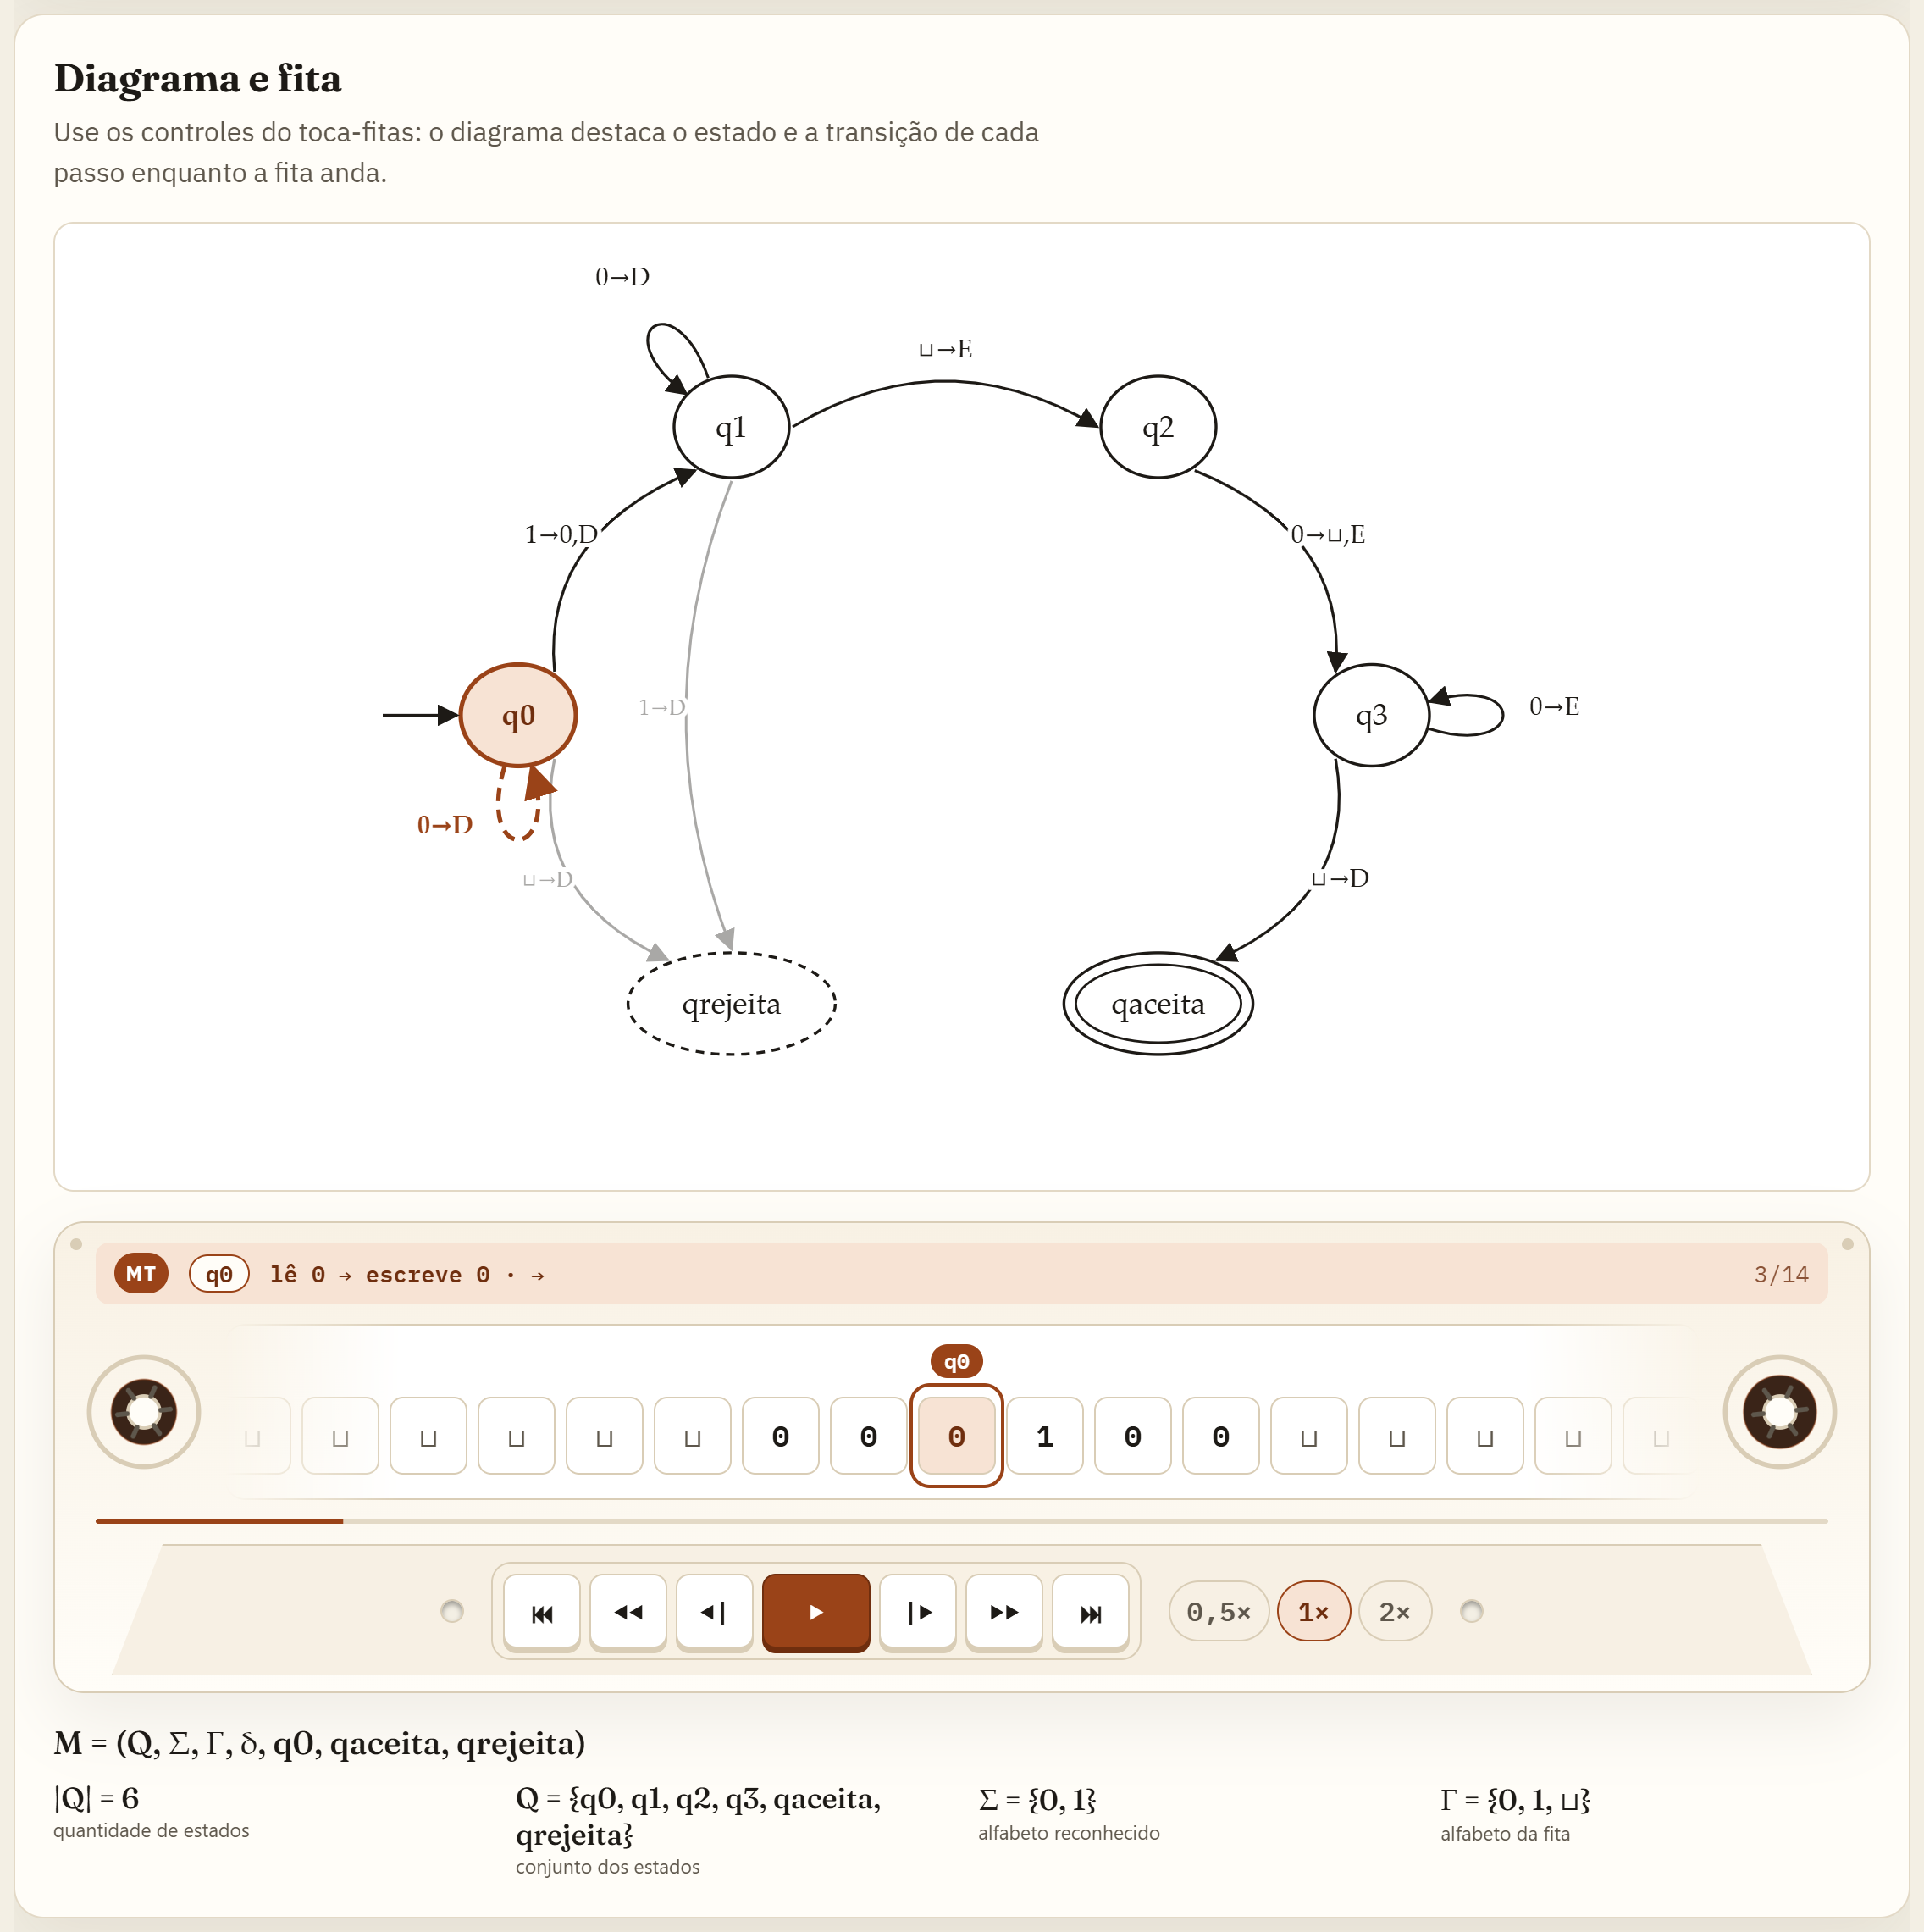
\includegraphics[width=0.82\textwidth]{figuras/tela-mt.png}
  \caption{Máquina de Turing da soma unária com a entrada $000100$, no
    terceiro passo: o diagrama destaca $q_0$ e o laço $0 \to D$, e a etiqueta
    da fita cassete mostra a regra aplicada (lê $0$, escreve $0$, move para a
    direita), com a célula lida sob o cabeçote.}
  \label{fig:tela-mt}
\end{figure}

\begin{figure}[htbp]
  \centering
  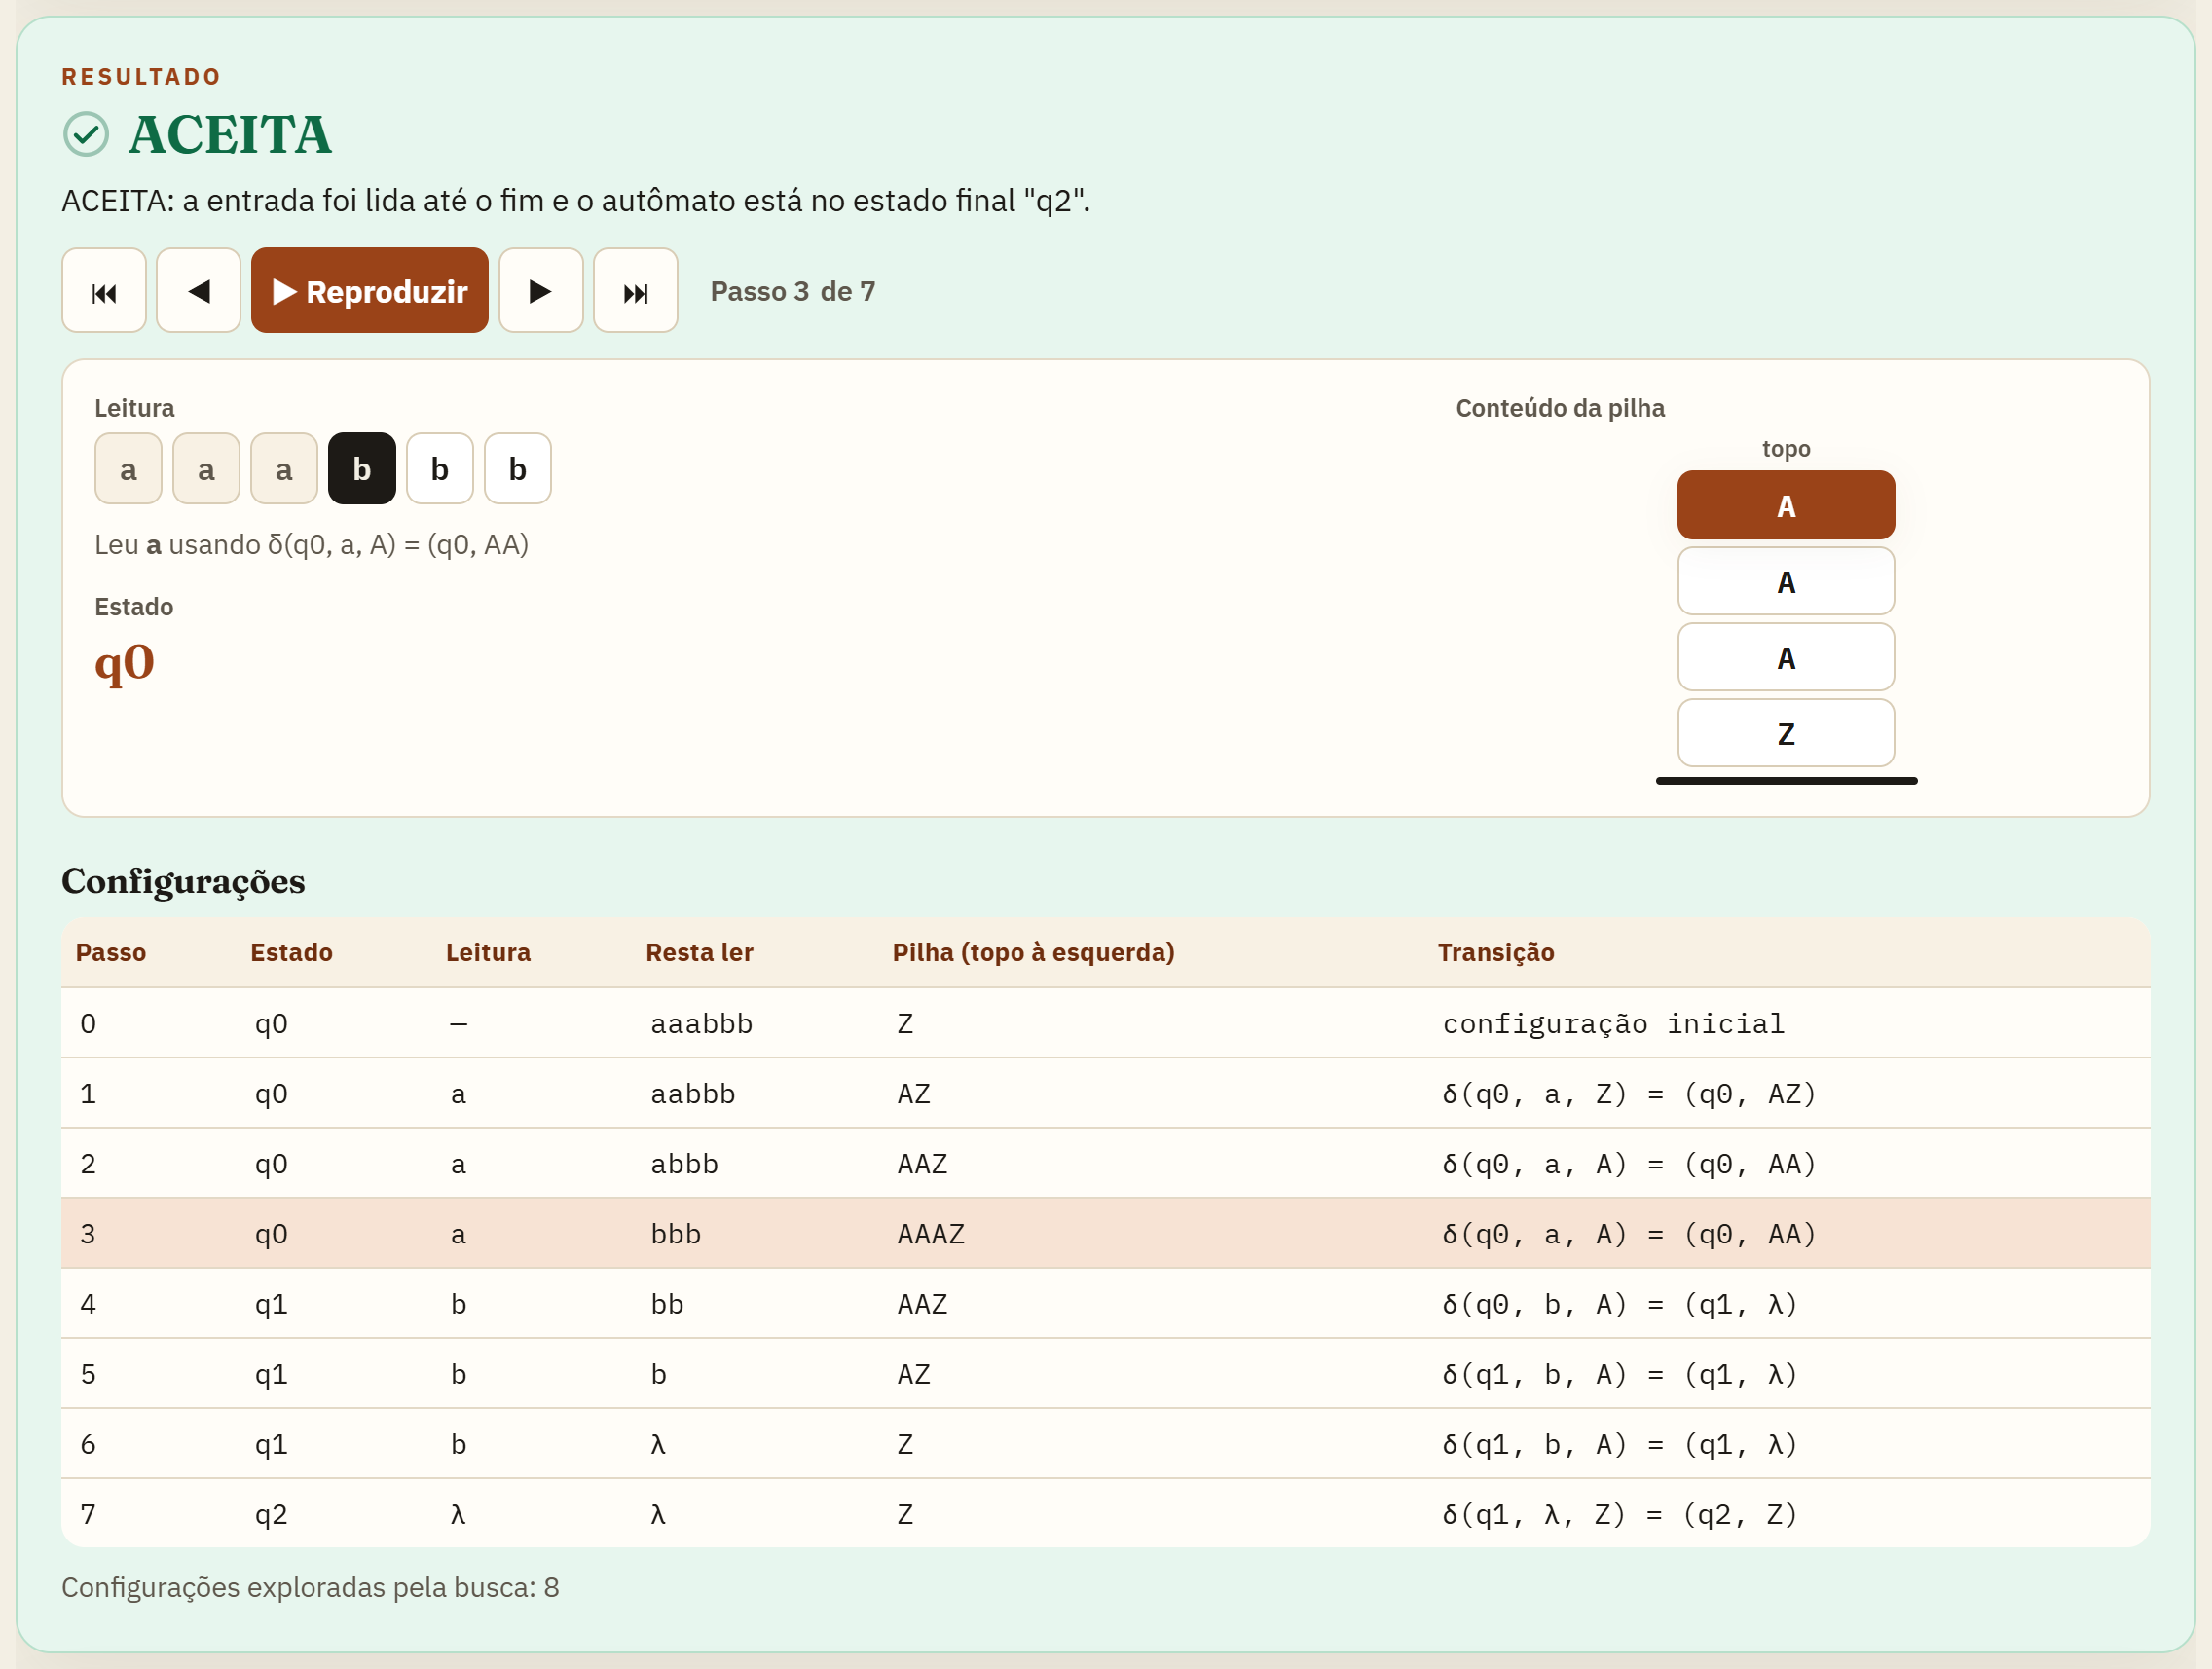
\includegraphics[width=0.82\textwidth]{figuras/tela-ap.png}
  \caption{Autômato com pilha de $\{a^nb^n \mid n \ge 1\}$ aceitando
    $aaabbb$, no terceiro passo: a cadeia lida, o estado atual, a pilha com o
    topo destacado e a tabela de configurações.}
  \label{fig:tela-ap}
\end{figure}

Para a fita deslizar sem saltos, cada célula precisa de uma posição que não
mude entre os retratos. Isso não é imediato, pois quando o cabeçote sai pela
esquerda da fita o \textit{backend} insere um branco na posição 0 e todos os
índices aumentam. Sendo $e_i$ o número de inserções à esquerda antes do
retrato $i$ e $E$ o total, a célula de índice $j$ no retrato $i$ recebe a
posição global $g = j - e_i + E$, a mesma em todos os retratos. Calcular os
$e_i$ custa $\Theta(p)$ para $p$ passos.

Isso cumpre o bônus do enunciado: interface gráfica em React exibindo
visualmente os estados dos autômatos, a pilha do AP e a fita da Máquina de
Turing.

\subsection{Testes e execução}

A Tabela~\ref{tab:testes} resume os testes automatizados (JUnit 5), que
cobrem os exemplos do enunciado e casos de erro. Para executar o sistema são
necessários o JDK 25 e o Node.js 18 ou superior:

{\small
\begin{verbatim}
cd frontend && npm install && npm run build  # gera a interface
cd ../backend && ./mvnw test                 # roda os 40 testes
./mvnw spring-boot:run                       # http://localhost:8080
\end{verbatim}}

\begin{table}[htbp]
  \centering
  \caption{Testes automatizados por módulo (40 no total, todos passando em Java 25).}
  \label{tab:testes}
  \small
  \begin{tabularx}{\textwidth}{lcX}
    \toprule
    Classe de teste & Testes & Exemplos verificados \\
    \midrule
    \cod{AnalisarLinguagemTest}     & 6  & $\Sigma=\{a,b\}$, $abba$: válida, tamanho 4; $\Sigma^*$ até $k=2$; $w\cdot v$ \\
    \cod{SimularAutomatoFinitoTest} & 7  & $ab$: $q_0 \to q_1 \to q_2$ aceita; AFN ``termina em $ab$''; AFN com $\lam$ \\
    \cod{DerivarCadeiaTest}         & 6  & $S \to aSb \mid \lam$ aceita $aaabbb$, rejeita $aab$; parênteses balanceados \\
    \cod{SimularAutomatoPilhaTest}  & 5  & $a^nb^n$ aceita $aabb$, rejeita $aab$, $abb$, $ba$, $\lam$; $ww^R$ \\
    \cod{SimularMaquinaTuringTest}  & 12 & soma unária $000100 \mapsto 00000$; $w\#w$ aceita $01\#01$, rejeita $01\#10$ \\
    \cod{ArquiteturaTest}           & 3  & regra de dependência entre as camadas (Seção~\ref{sec:arquitetura}) \\
    Contexto Spring                 & 1  & a aplicação sobe \\
    \bottomrule
  \end{tabularx}
\end{table}

% ====================================================== 5 complexidade
\section{Análise de complexidade}

\subsection{Notação}

Para funções $f, g: \mathbb{N} \to \mathbb{R}^+$ \cite{cormen}:
$f(n) = O(g(n))$ se existem $c > 0$ e $n_0$ tais que $f(n) \le c\,g(n)$ para
todo $n \ge n_0$ (limite superior); $f(n) = \Omega(g(n))$ se
$f(n) \ge c\,g(n)$ a partir de algum $n_0$ (limite inferior); e
$f(n) = \Theta(g(n))$ se ambos valem (limite justo). Abaixo, $n = |w|$; o
tamanho do modelo ($|Q|$, $|\delta|$, $|P|$) é tratado como constante, salvo
quando aparece na fórmula. Consultas a \cod{HashSet} e \cod{HashMap} custam
$O(1)$ esperado.

\subsection{Análise por algoritmo}

\paragraph{Validação de $w \in \Sigma^*$.} Uma consulta por símbolo. Melhor
caso $\Omega(1)$ (o primeiro símbolo está fora de $\Sigma$); pior caso e caso
médio de uma cadeia válida $\Theta(n)$. O tamanho $|w|$ custa $\Theta(1)$, pois
a \cod{String} Java guarda seu comprimento, e a concatenação $w \cdot v$ custa
$\Theta(|w| + |v|)$, pela cópia dos símbolos.

\paragraph{Listagem de $\Sigma^*$ até $k$.} São $\sum_{i=0}^{k} |\Sigma|^i$
cadeias, cada uma com até $k$ símbolos, logo $\Theta(k\,|\Sigma|^k)$ para
$|\Sigma| \ge 2$ em todos os casos: exponencial em $k$, o que justifica o teto
de 500 itens.

\paragraph{Simulação de AFD.} Uma consulta $\delta(q, a)$ por símbolo:
$\Theta(n)$ quando a cadeia é lida até o fim; $\Omega(1)$ no melhor caso, se
falta transição logo no início.

\paragraph{Simulação de AFN.} Em cada um dos $n$ passos, a união percorre no
máximo $|Q|$ estados e suas transições, e o fecho-$\lam$ é uma busca em
profundidade em $O(|Q| + |\delta|)$. Logo o pior caso é
$O(n\,(|Q| + |\delta|)) \subseteq O(n\,|Q|^2|\Sigma|)$, linear em $n$; o melhor
caso é $\Omega(n)$ (um estado ativo por vez). Converter o AFN em AFD antes
custaria $O(2^{|Q|})$ estados, o que a simulação por conjuntos evita.

\paragraph{Derivação em GLC.} Cada forma sentencial tem tamanho $O(n)$ pela poda
(iv), e montá-la custa $O(n)$. No melhor caso, só uma produção é viável por
passo: para $S \to aSb \mid \lam$ e $w = a^mb^m$, a busca visita $O(n)$ formas,
logo $\Omega(n^2)$. No pior caso, com fator de ramificação $b$ (máximo de
alternativas por variável) e derivações de tamanho $d = O(n)$, são até $b^d$
formas, ou seja $O(b^d \cdot n)$: exponencial. O desempenho médio depende da
gramática e é bom para gramáticas pouco ambíguas, como as dos exemplos. Uma
alternativa polinomial é o algoritmo CYK, $\Theta(n^3\,|G|)$, que exige a
gramática na Forma Normal de Chomsky; a busca foi preferida por produzir
diretamente a derivação passo a passo e a árvore pedidas.

\paragraph{Simulação de AP.} O número de configurações distintas é limitado por
$|Q| \cdot (n+1) \cdot \sum_{h \le H} |\Gamma|^h$, com $H = 2n + 10$, e cada uma
custa $O(|\delta| + n)$ (testar as regras e copiar a pilha). O pior caso é
portanto exponencial, $O(|Q|\,n\,|\Gamma|^{H})$. Para um AP determinístico,
como o de $a^nb^n$, existe um único caminho com $O(n)$ configurações:
$\Omega(n)$ passos; na implementação, a cópia da pilha (\cod{String}) faz o
custo total ser $O(n^2)$, que cairia para $\Theta(n)$ com uma pilha mutável.

\paragraph{Máquina de Turing (laço genérico).} Cada passo procura a regra
percorrendo $\delta$, em $O(|\delta|)$, e registra a fita, em $O(t)$, sendo $t$ o
tamanho da fita; com $p$ passos, o custo é $O(p\,(|\delta| + t))$, limitado pelo
teto de 2\,000 passos. O melhor caso é $\Omega(1)$, quando o estado inicial
já é de aceitação.

\paragraph{MT da soma unária.} Para $w = 0^a10^b$, com $n = a + b + 1$, a máquina
anda $n+1$ células para a direita, apaga um $0$ e volta $n$ células: exatamente
$2n + 2$ passos (14 para $000100$). Logo $\Theta(n)$ nos três casos.

\paragraph{MT de $w\#w$.} Seja $m = |w|$, de modo que $n = 2m + 1$. Para cada um
dos $m$ símbolos de $w$, a máquina vai até o símbolo correspondente depois do
$\#$ e volta, percorrendo $\Theta(m)$ células; o total é $\Theta(m^2) =
\Theta(n^2)$ quando a cadeia é aceita (pior caso e caso médio). No melhor caso
o primeiro par já difere e a máquina para após uma ida: $\Omega(n)$.

\begin{table}[htbp]
  \centering
  \caption{Resumo da análise assintótica ($n = |w|$).}
  \label{tab:complexidade}
  \small
  \begin{tabular}{llll}
    \toprule
    Algoritmo & Melhor caso & Caso médio & Pior caso \\
    \midrule
    Validar $w \in \Sigma^*$ & $\Omega(1)$ & $\Theta(n)$ & $O(n)$ \\
    Tamanho $|w|$ & $\Theta(1)$ & $\Theta(1)$ & $\Theta(1)$ \\
    Concatenação $w \cdot v$ & $\Theta(|w|+|v|)$ & $\Theta(|w|+|v|)$ & $\Theta(|w|+|v|)$ \\
    Listar $\Sigma^*$ até $k$ & $\Theta(k|\Sigma|^k)$ & $\Theta(k|\Sigma|^k)$ & $\Theta(k|\Sigma|^k)$ \\
    AFD & $\Omega(1)$ & $\Theta(n)$ & $O(n)$ \\
    AFN por conjuntos & $\Omega(n)$ & $\Theta(n|Q|)$ & $O(n(|Q|+|\delta|))$ \\
    GLC (busca em largura) & $\Omega(n^2)$ & depende de $G$ & $O(b^d n)$ \\
    GLC (CYK, alternativa) & $\Theta(n^3|G|)$ & $\Theta(n^3|G|)$ & $\Theta(n^3|G|)$ \\
    AP (busca em largura) & $\Omega(n)$ & depende de $M$ & $O(|Q|\,n\,|\Gamma|^{2n+10})$ \\
    MT: soma unária & $\Theta(n)$ & $\Theta(n)$ & $\Theta(n)$ \\
    MT: $w\#w$ & $\Omega(n)$ & $\Theta(n^2)$ & $O(n^2)$ \\
    \bottomrule
  \end{tabular}
\end{table}

% ======================================================= 6 conclusão
\section{Conclusão}

O simulador cobre os cinco modelos pedidos e mostra, para cada um, o
processamento passo a passo e o diagrama do modelo, o que permite observar na
prática conceitos que em sala aparecem só no papel: o conjunto de estados
ativos do AFN, a derivação e a árvore de uma GLC, a pilha de um AP e a fita
de uma MT. A análise de complexidade evidencia a hierarquia entre os
modelos: os autômatos finitos são simulados em tempo linear, enquanto o
reconhecimento por busca em GLCs e APs não determinísticos pode ser
exponencial no pior caso, e uma MT pode nem parar. Esse custo foi controlado
com podas e tetos de busca.

Como trabalhos futuros, destacam-se: implementar o algoritmo CYK (ou Earley)
para garantir tempo polinomial nas GLCs; converter AFN em AFD e minimizar
autômatos; e permitir máquinas de Turing com várias fitas.

As principais dificuldades foram garantir que as buscas não determinísticas
(GLC e AP) sempre terminassem sem rejeitar cadeias válidas, o que levou às
podas por prefixo, sufixo e variáveis anuláveis; desenhar automaticamente
diagramas de estados legíveis para qualquer autômato digitado pelo usuário; e
separar o código em camadas sem que o domínio dependesse da validação da
entrada. A principal lição foi que implementar cada modelo obriga a tornar
precisa cada parte da definição formal: o que acontece quando falta uma
transição, quando a pilha esvazia ou quando a máquina não para.

\paragraph{Código-fonte.} O repositório traz instruções de execução e
exemplos de entrada e saída no \cod{README}:\\
\url{https://github.com/lpeixotomagalhaes/simulador-linguagens-formais}

% ===================================================== referências
\begingroup\small\setstretch{1.15}
\begin{thebibliography}{9}
  \bibitem{cormen} CORMEN, T. H.; LEISERSON, C. E.; RIVEST, R. L.; STEIN, C.
    \textit{Algoritmos: teoria e prática}. 3. ed. Rio de Janeiro: Elsevier, 2012.
  \bibitem{hopcroft} HOPCROFT, J. E.; MOTWANI, R.; ULLMAN, J. D.
    \textit{Introdução à teoria de autômatos, linguagens e computação}.
    Rio de Janeiro: Campus, 2002.
  \bibitem{menezes} MENEZES, P. B. \textit{Linguagens formais e autômatos}.
    6. ed. Porto Alegre: Bookman, 2011.
  \bibitem{sipser} SIPSER, M. \textit{Introdução à teoria da computação}.
    2. ed. São Paulo: Cengage Learning, 2007.
\end{thebibliography}
\endgroup

\end{document}
